\chapter{Simulation}
\label{simulation}

\section{Introduction}

A series of simulation experiments was performed.  Below is the list
of nine experiments.  Each experiment generated a sample trace of
length 1,000 seconds.

\begin{enumerate}
\item	Poisson process simulation.
\item	Renewal process with scaled uniform inter-renewal distribution.
\item	A 3-state modulated renewal process.
\item	Renewal process with Pareto (infinite variance) inter-renewal distribution.
\item	Renewal process with $t_2-distribution$ (infinite variance) inter-renewal distribution.
\item	Renewal process with Cauchy inter-renewal (infinite variance) distribution.
\item	Single renewal process with $t_2-distribution$ inter-renewal distribution.
\item	10 super-imposed independent renewal processes with $t_2-distribution$ inter-renewal distributions.
\item	100 super-imposed independent renewal processes with $t_2-distribution$ inter-renewal distributions.
\end{enumerate}

The simulations were done using a single chain of recurrent events,
ordered by time.  Each event is independent of all others on the
chain, and knows when in the future it will occur.  The chain also has
a notion of the current time.  When an event reaches the head of the
chain it occurs and is recorded into the trace file.  The current time
is set to the time of the event and a new time for it to occur is
generated.  This event (now to occur sometime in the future) is placed
back into the chain in chronological order.

The events are self contained and may have simple (samples from some
distribution) or complex (with multiple internal states) recurrent
behaviour.  All that is required is that it generates a new recurrence
time in the positive future.

\section{Simulation of simple Poisson process}
\label{simulation:simplepp}

Using the simplest model available, that is exponentially distributed
inter-arrival times, we can produce sample traces to examine.  This
simulation is not meant to be comparable to the real traces, but
rather a counter example to show that such a model does not fit
Ethernet traffic patterns.

It is also intended to show that the simulation techniques work
properly and that the tools developed to produce the results are
robust.

\subsection{Exponential arrival distribution}

\begin{figure}
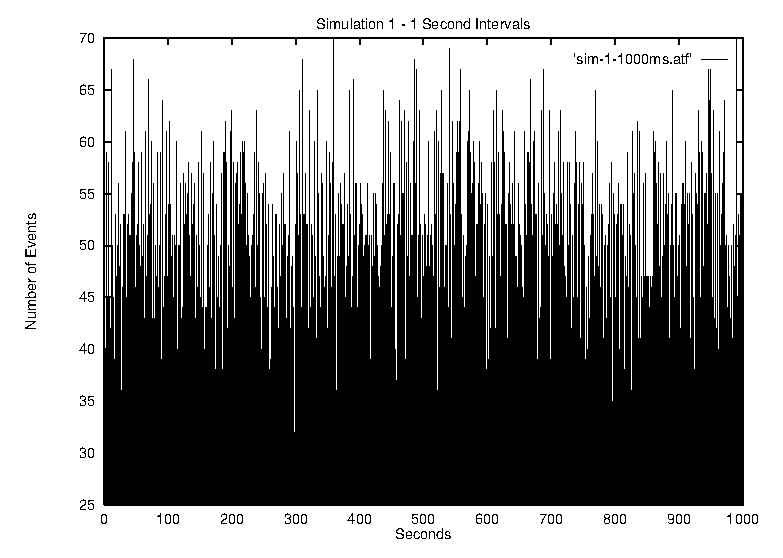
\includegraphics[height=3in]{pics/sim-1-1s-freq.eps}
\caption{Poisson Process Simulation with Exponential Distribution}
\label{simulation:sim1.1s.freq}
\end{figure}

\begin{figure}
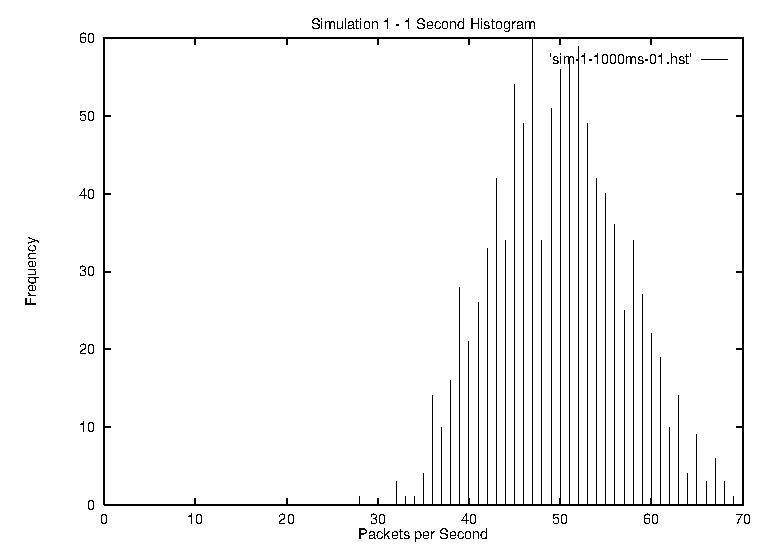
\includegraphics[height=3in]{pics/sim-1-1s-hist-01.eps}
\caption{Histogram of a Poisson Process Simulation}
\label{simulation:sim1.1s.hist}
\end{figure}

\begin{figure}
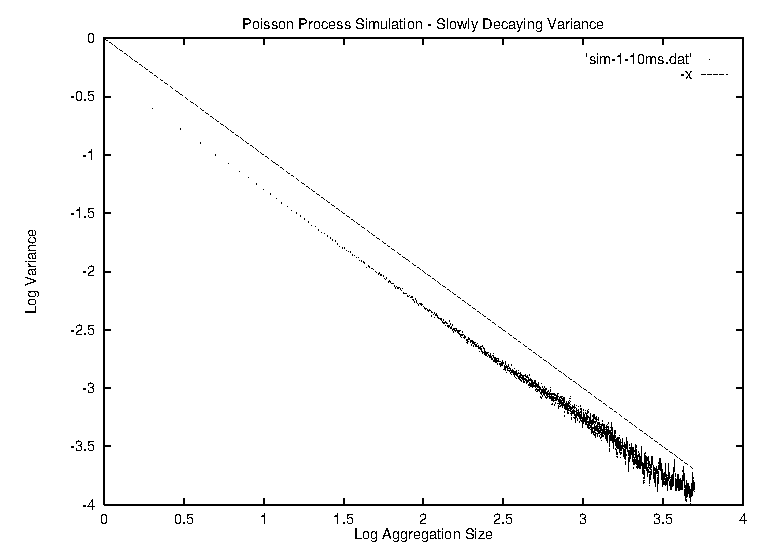
\includegraphics[height=3in]{pics/sim-1-10ms-sta.eps}
\caption{Slowly decaying variance plot of a Poisson Process Simulation}
\label{simulation:sim1.10ms.sta}
\end{figure}

The first simulation {\em sim-1} is a Poisson Process with rate
$\lambda = 0.05$ packets per millisecond, simulated over a period of
1,000 seconds ($\sim$ 16 minutes).  This results in an exponentially
distributed inter-arrival time with mean $\mu = 20$.  A sample trace
can be seen in figure~\ref{simulation:sim1.1s.freq} along with the
packet frequency histogram (figure~\ref{simulation:sim1.1s.hist}) and
slowly decaying variance plot
(figure~\ref{simulation:sim1.10ms.sta}).  As expected the plot is a
straight line with a slope of $-1$, hence the variance decays order
$n^{-1}$ with averaging aggregation, in line with the theoretical
model.

\subsection{Single state with uniform inter-arrival time distribution}

\begin{figure}
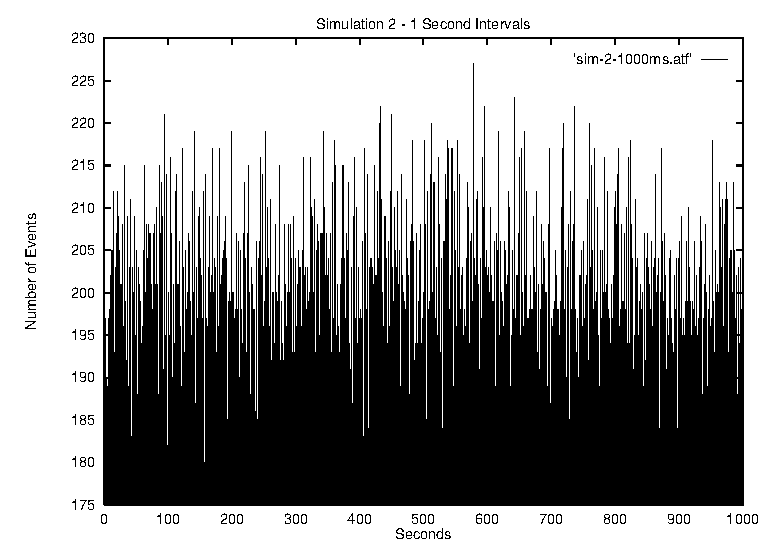
\includegraphics[height=3in]{pics/sim-2-1s-freq.eps}
\caption{Uniform Distribution Renewal Process Simulation}
\label{simulation:sim2.1s.freq}
\end{figure}

\begin{figure}
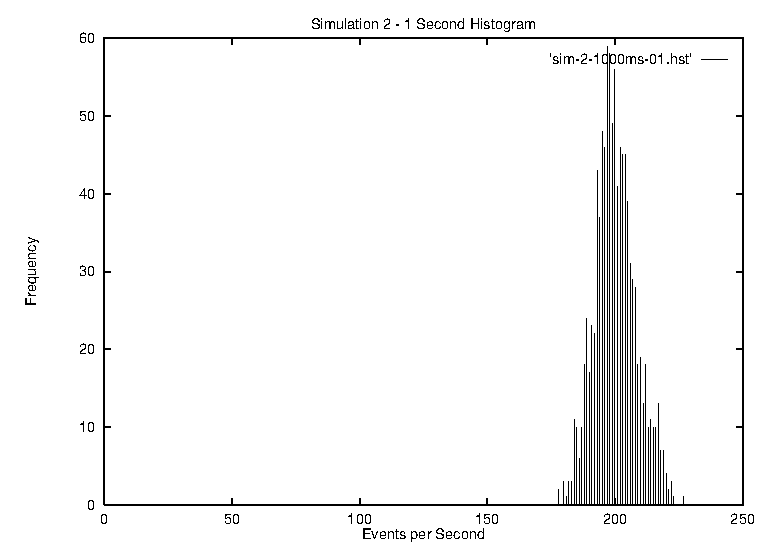
\includegraphics[height=3in]{pics/sim-2-1s-hist-01.eps}
\caption{Histogram of Uniform Distribution Renewal Process Simulation}
\label{simulation:sim2.1s.hist}
\end{figure}

\begin{figure}
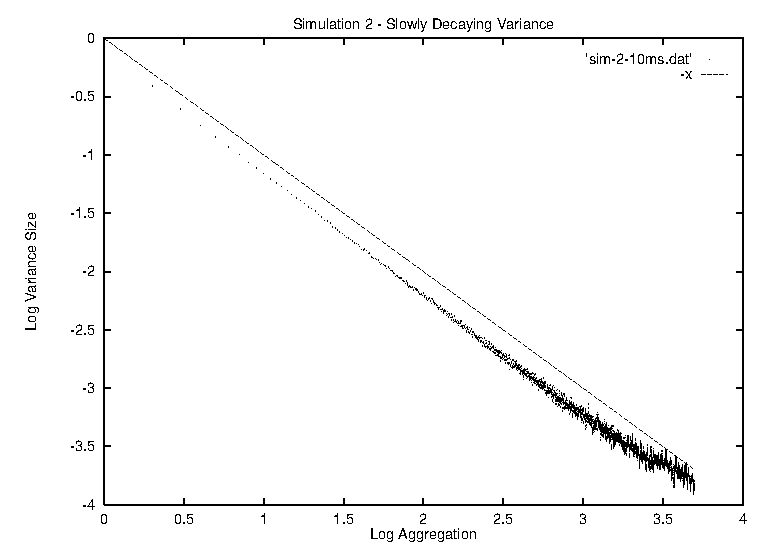
\includegraphics[height=3in]{pics/sim-2-10ms-sta.eps}
\caption{Slowly decaying variance plot of Uniform Distribution Renewal Process Simulation}
\label{simulation:sim2.10ms.sta}
\end{figure}

The second simulation \emph{sim-2} is a renewal process which has
inter-arrival times that are uniformly distributed with mean $\mu =
20$.  The time series can be seen in
figure~\ref{simulation:sim2.1s.freq} along with its histogram
(figure~\ref{simulation:sim2.1s.hist}) and the slowly decaying
variance plot (figure~\ref{simulation:sim2.10ms.sta}).  Again the
variance plot is a straight line with slope $-1$, that is it shows no
sign of self-similar behaviour.

\section{Generalised modulated renewal process}

\subsection{The model}

The mathematical model for this simulation is discussed in the models
chapter (\S \ref{models:genmodproc}).

\subsection{The program}

The program reads in a parameter file and produces a trace file
(Figure~\ref{trace:format}).

{\ttfamily \begin{flushleft}
  simulate [-t time in seconds] parameter files
\end{flushleft}}

\subsubsection{An example}

For an example I have chosen a three state process.

\bigskip

\begin{tabular}{||l||l|l||l|l||} \hline
State & \multicolumn{2}{l||}{Inter-Event Distribution} &
\multicolumn{2}{l||}{Lifetime Distribution} \\ \hline
 & Distribution & Mean & Distribution & Mean \\ \hline \hline
0 & Exponential & 10 & Exponential & 100 \\ \hline
1 & Deterministic & 2 & Uniform & 40 \\ \hline
2 & Deterministic & 1 & Deterministic & 15 \\ \hline
\end{tabular}

\bigskip

\begin{figure}
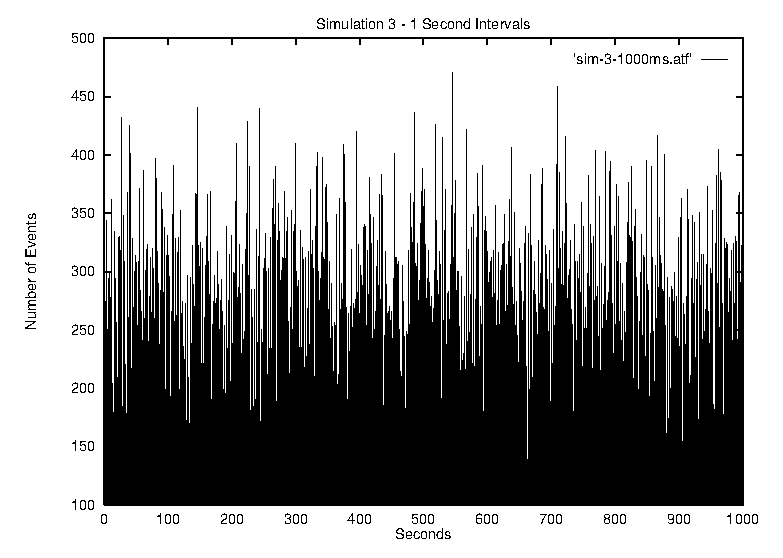
\includegraphics[height=3in]{pics/sim-3-1s-freq.eps}
\caption{Modulated Renewal Process Simulation}
\label{simulation:sim3.1s.freq}
\end{figure}

\begin{figure}
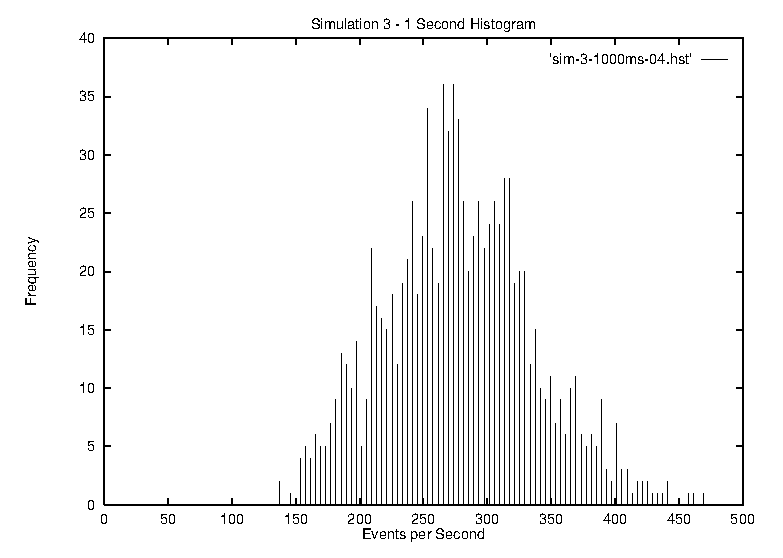
\includegraphics[height=3in]{pics/sim-3-1s-hist-04.eps}
\caption{Histogram of Modulated Renewal Process Simulation}
\label{simulation:sim3.1s.hist}
\end{figure}

\begin{figure}
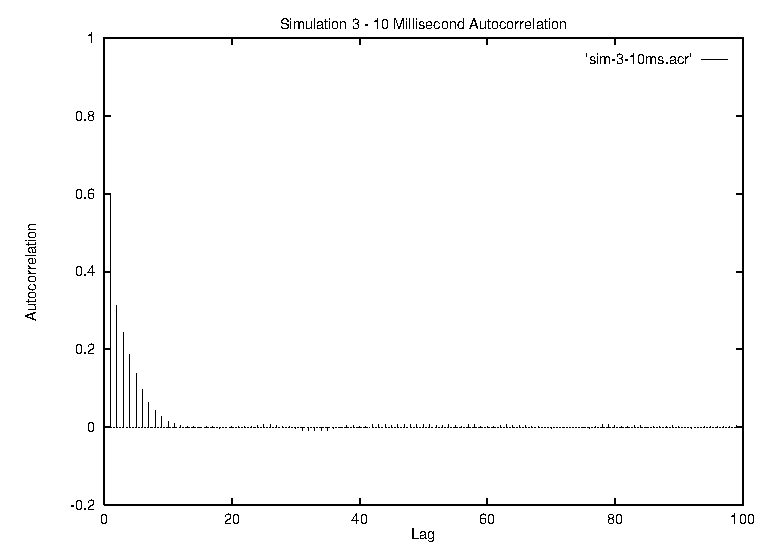
\includegraphics[height=3in]{pics/sim-3-10ms-acr.eps}
\caption{Autocorrelation of Modulated Renewal Process Simulation}
\label{simulation:sim3.10ms.acr}
\end{figure}

\begin{figure}
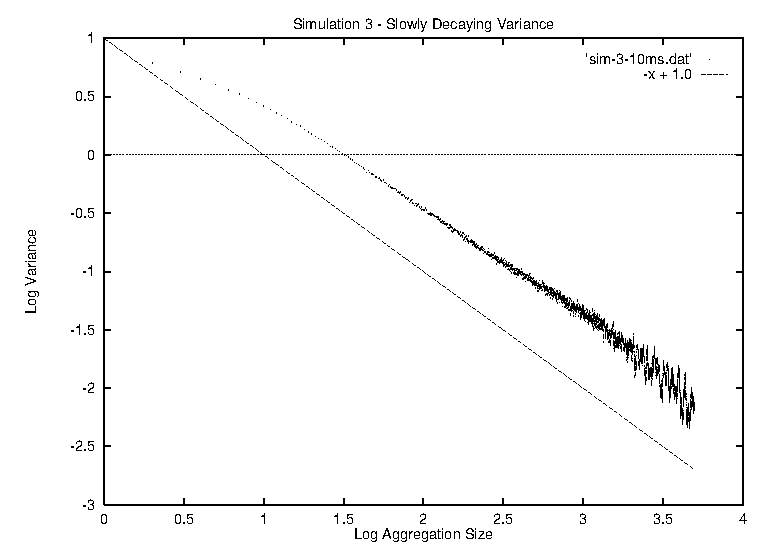
\includegraphics[height=3in]{pics/sim-3-10ms-sta.eps}
\caption{Slowly decaying variance plot of Modulated Renewal Process Simulation}
\label{simulation:sim3.10ms.sta}
\end{figure}

The results of the simulation \emph{sim-3} are shown in figures
\ref{simulation:sim3.1s.freq}, \ref{simulation:sim3.1s.hist},
\ref{simulation:sim3.10ms.acr} and \ref{simulation:sim3.10ms.sta}.
The time series (figure \ref{simulation:sim3.1s.freq}) looks bursty
but the histogram (figure \ref{simulation:sim3.1s.hist} shows that the
number of large bursts is small and that most of the flows are in a
limited range (200 -- 350 events per second).

The autocorrelation (figure \ref{simulation:sim3.10ms.acr}) shows the
existence of a definite short term correlation, caused by the
deterministic behaviour within two of the states.  This short term
correlation falls away in relation to the expected life time of the
deterministic states to white noise caused by the Poisson distributed
state and life time.

The slowly decaying variance graph (figure
\ref{simulation:sim3.10ms.sta}) shows that this model is not what we
are looking for, and that a more complex model does not help.

\clearpage

\section{Infinite variance renewal processes}

\subsection{Introduction}

Below are the results of three simple renewal processes, similar to
the simple Poisson process (\S \ref{simulation:simplepp}) except that
the inter-renewal distributions have infinite variance.  This class
(having infinite variance) of distributions is often known as
heavy-tailed distributions.

The three distributions used are the Pareto distribution, a non
symmetric distribution that is defined on ${\mathbb R}^+$.  This
distribution was used because of its reference in \cite{Bell:4} (\S
3.2.3, Page 19).  The Pareto distribution is a stable distribution
making further mathematical analysis a little simpler than other
distributions.

The other two distributions come from Student's $t$ distribution.  For
degrees of freedom 1 and 2 it has infinite variance.  The
$t_1-distribution$, commonly known as the Cauchy distribution, also
has infinite mean.  The $t_\nu-distribution$ is a flattened normal,
symmetric and defined on all of ${\mathbb R}$.  For the simulations
the distributions are folded around the y-axis so that only positive
inter-renewal times exist.

\subsection{Pareto distribution}

\begin{figure}
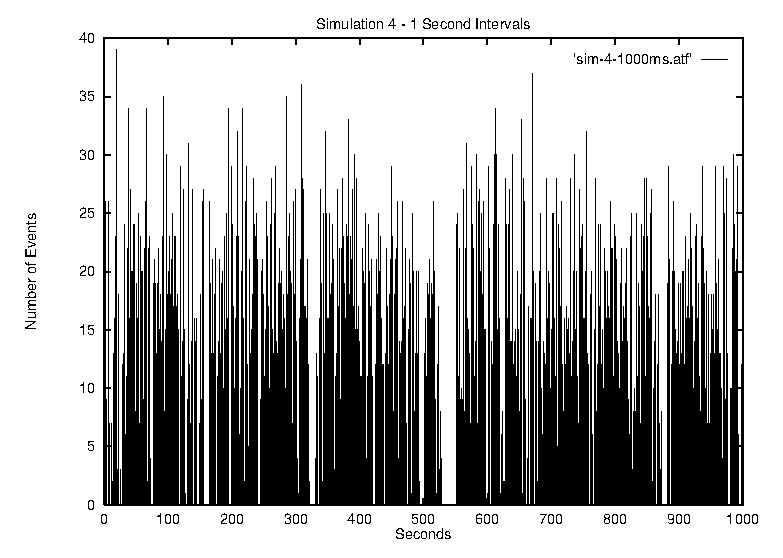
\includegraphics[height=3in]{pics/sim-4-1s-freq.eps}
\caption{Pareto Distributed Renewal Process Simulation}
\label{simulation:sim4.1s.freq}
\end{figure}

\begin{figure}
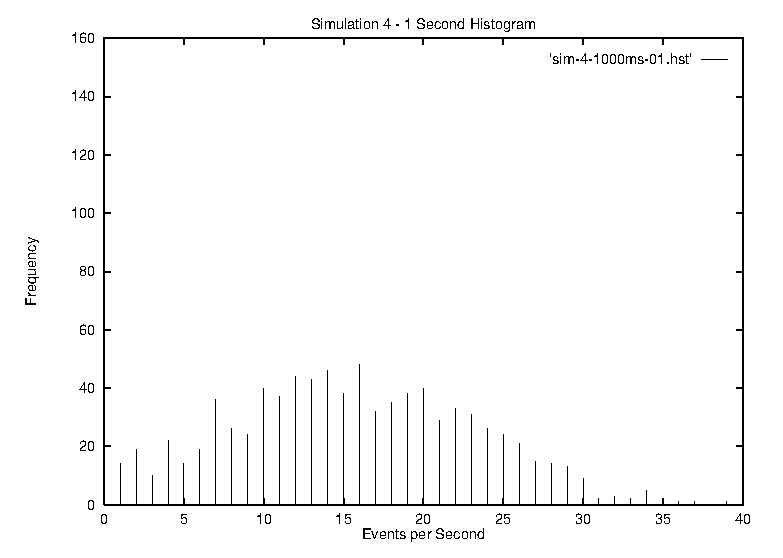
\includegraphics[height=3in]{pics/sim-4-1s-hist-01.eps}
\caption{Histogram of Pareto Distributed Renewal Process Simulation}
\label{simulation:sim4.1s.hist}
\end{figure}

\begin{figure}
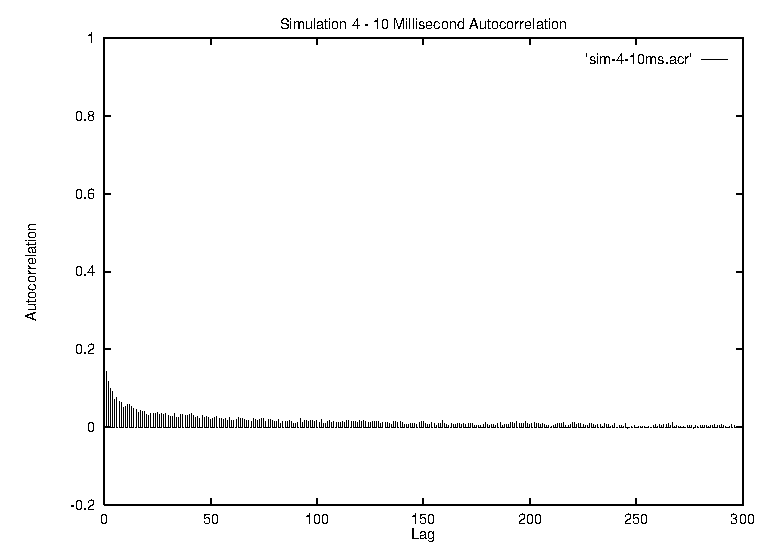
\includegraphics[height=3in]{pics/sim-4-10ms-acr.eps}
\caption{Autocorrelation of Pareto Distributed Renewal Process Simulation}
\label{simulation:sim4.10ms.acr}
\end{figure}

\begin{figure}
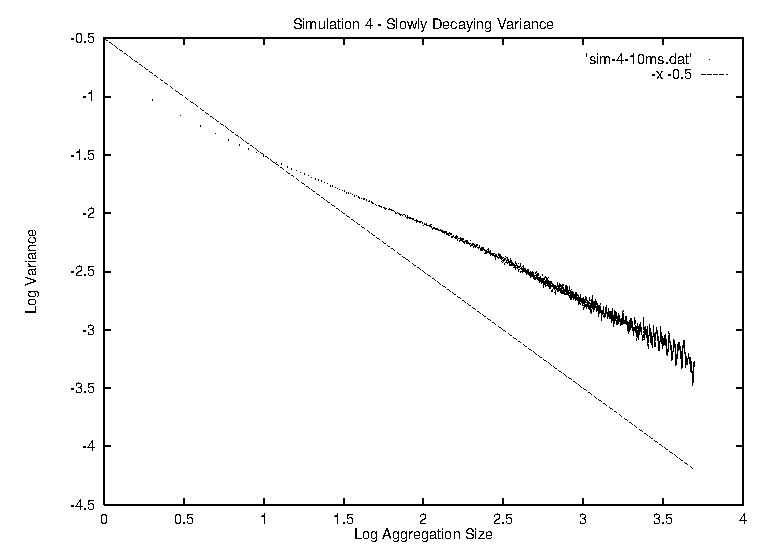
\includegraphics[height=3in]{pics/sim-4-10ms-sta.eps}
\caption{Slowly decaying variance plot of Pareto Distributed Renewal Process Simulation}
\label{simulation:sim4.10ms.sta}
\end{figure}

The time series for \emph{sim-4} is shown in figure
\ref{simulation:sim4.1s.freq}.  The large number of gaps and lack of
``background'' traffic are notable features of this plot (the
$t-distribution$ plots also show this behaviour).  The histogram
(figure \ref{simulation:sim4.1s.hist}) shows a wide range of traffic
levels.  Note that although it cannot be seen there is bar of height
143 at 0 events per second.

The autocorrelation (figure \ref{simulation:sim4.10ms.acr}) displays
the important positive autocorrelation, indicating long range
dependence.  The slowly decaying variance (figure
\ref{simulation:sim4.10ms.sta}) shows the decay occuring at a slower
rate than $x^{-1}$, verifying that infinite variance renewal processes
do exhibit fractal behaviour.

\subsection{Cauchy and $t$ distributions}

\begin{figure}[h]
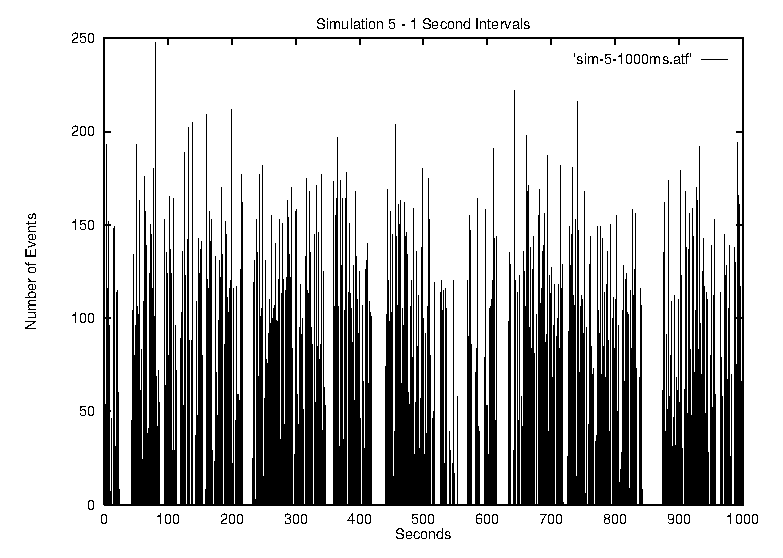
\includegraphics[height=3in]{pics/sim-5-1s-freq.eps}
\caption{$t_2-distribution$ Distributed Renewal Poisson Simulation}
\label{simulation:sim5.1s.freq}
\end{figure}

\begin{figure}
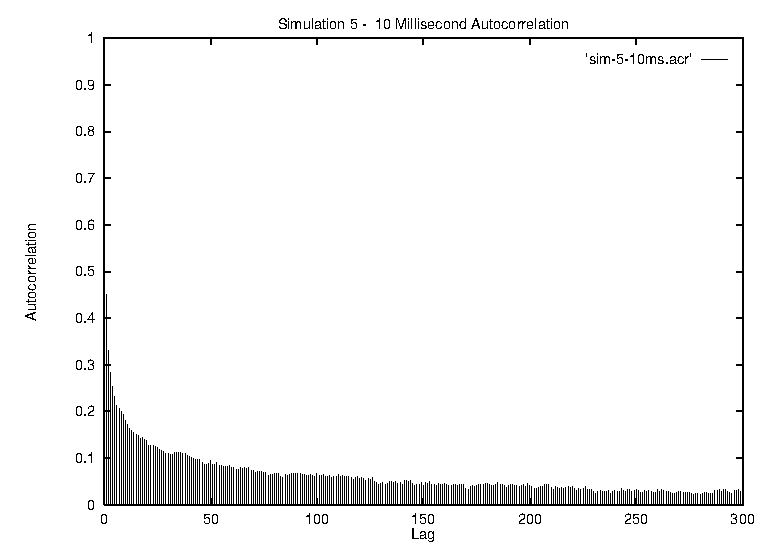
\includegraphics[height=3in]{pics/sim-5-10ms-acr.eps}
\caption{Autocorrelation of $t_2-distribution$ Distributed Renewal Process Simulation}
\label{simulation:sim5.10ms.acr}
\end{figure}

\begin{figure}
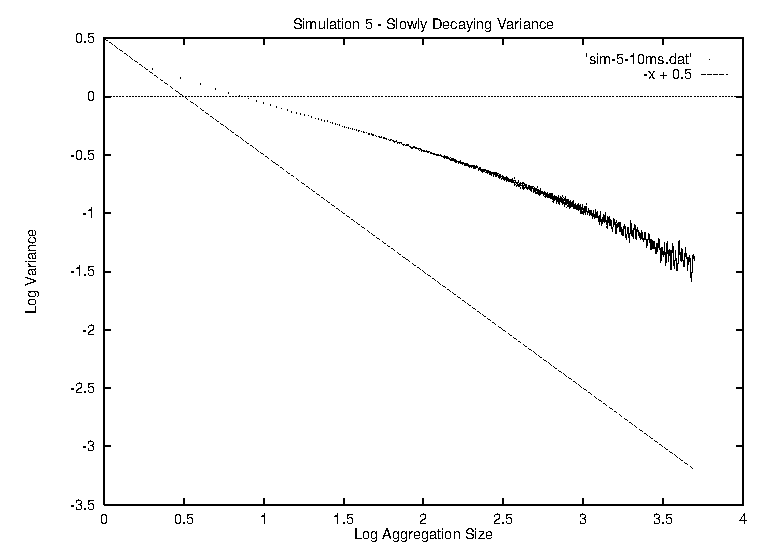
\includegraphics[height=3in]{pics/sim-5-10ms-sta.eps}
\caption{Slowly decaying variance plot of $t_2-distribution$ Distributed Renewal Process Simulation}
\label{simulation:sim5.10ms.sta}
\end{figure}


\begin{figure}
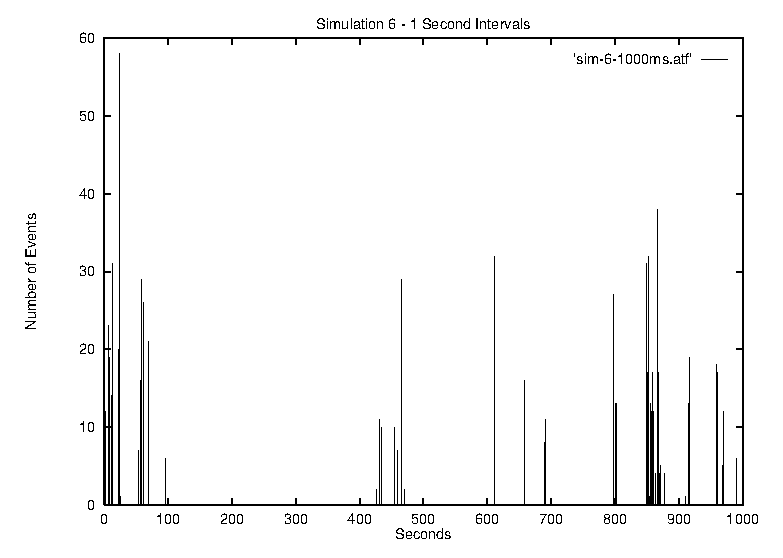
\includegraphics[height=3in]{pics/sim-6-1s-freq.eps}
\caption{Cauchy Distributed Renewal Poisson Simulation}
\label{simulation:sim6.1s.freq}
\end{figure}

\begin{figure}
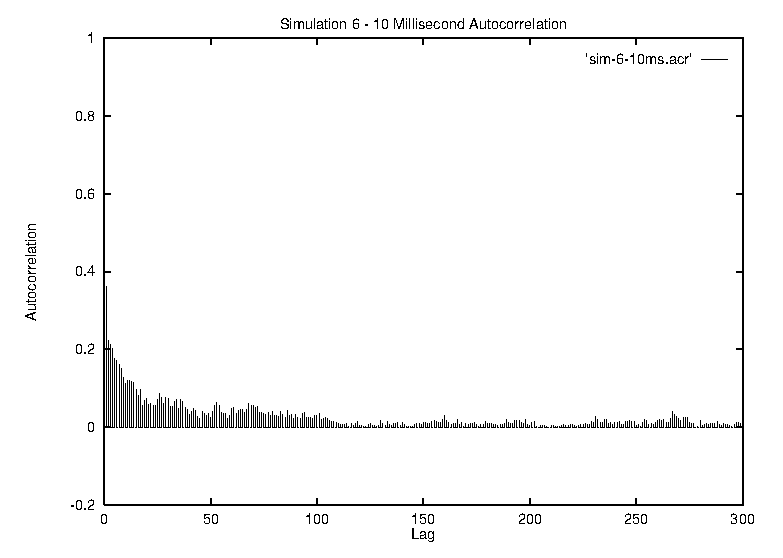
\includegraphics[height=3in]{pics/sim-6-10ms-acr.eps}
\caption{Autocorrelation of Cauchy Distributed Renewal Process Simulation}
\label{simulation:sim6.10ms.acr}
\end{figure}

\begin{figure}
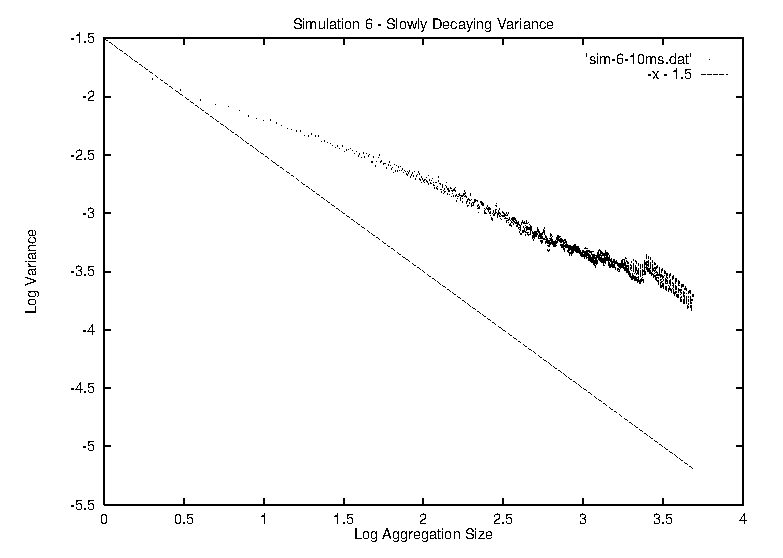
\includegraphics[height=3in]{pics/sim-6-10ms-sta.eps}
\caption{Slowly decaying variance plot of Cauchy Distributed Renewal Process Simulation}
\label{simulation:sim6.10ms.sta}
\end{figure}

Figures \ref{simulation:sim5.1s.freq}, \ref{simulation:sim5.10ms.acr}
and \ref{simulation:sim5.10ms.sta} are the result from simulating a
general renewal process with a $t_2-distribution$ inter-renewal
distribution (\emph{sim-5}).

Figures \ref{simulation:sim6.1s.freq}, \ref{simulation:sim6.10ms.acr}
and \ref{simulation:sim6.10ms.sta} are the result from simulating a
general renewal process with a Cauchy ($t_1-distribution$) inter-renewal
distribution (\emph{sim-6}).

The Cauchy distribution simulation generated very few (in comparison
with the other simulations and real samples) events so that the
analysis is less reliable.  The $t_2-distribution$ results show strong
positive autocorrelation and noticeable slowly decaying variance.

\clearpage

\subsection{Merged $t_2-distribution$ renewal processes}

Below are the results for the superimposed (or merged) renewal
processes.  The full definition can be found in the models chapter (\S
\ref{models:mergedprocs}).  The base distribution is a $t_2-distribution$.
This was used as it produced clear results in the earlier simulations.
The choice of the $t_2-distribution$ rather than Pareto was mainly one
of personal opinion and my impression that it gave a clearer results
with respect to slowly decaying variance and long range dependence
(the autocorrelation).  Earlier experiments show that the Pareto is a
perfectly acceptable distribution for these experiments and produces
similar conclusions.

A single process is repeated (identical in distribution to simulation
5) as a control (\emph{sim-7}). 10 and 100 merged processes were then
produced (\emph{sim-8} and \emph{sim-9} respectively).  Both of these
produced a large number of total events giving decisive results.

\begin{figure}[h]
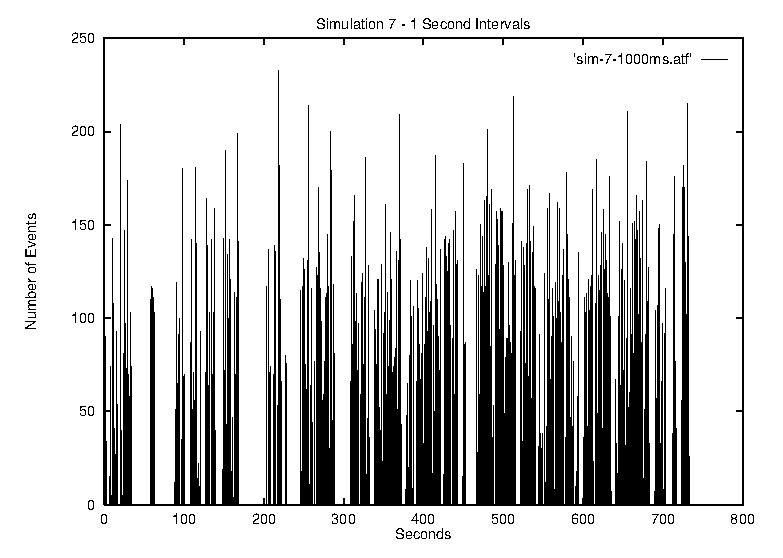
\includegraphics[height=3in]{pics/sim-7-1s-freq.eps}
\caption{Single $t_2-distribution$ Distributed Renewal Process Simulation}
\label{simulation:sim7.1s.freq}
\end{figure}

\begin{figure}
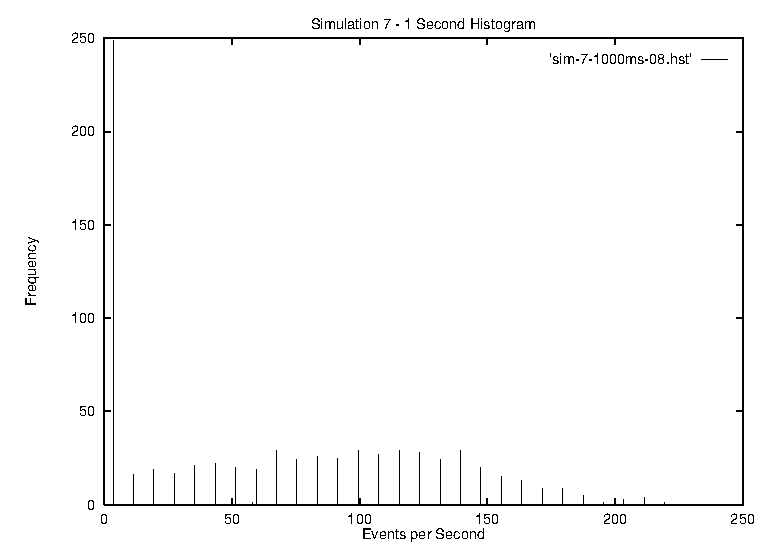
\includegraphics[height=3in]{pics/sim-7-1s-hist-08.eps}
\caption{Histogram of Single $t_2-distribution$ Distributed Renewal Process Simulation}
\label{simulation:sim7.1s.hist}
\end{figure}

\begin{figure}
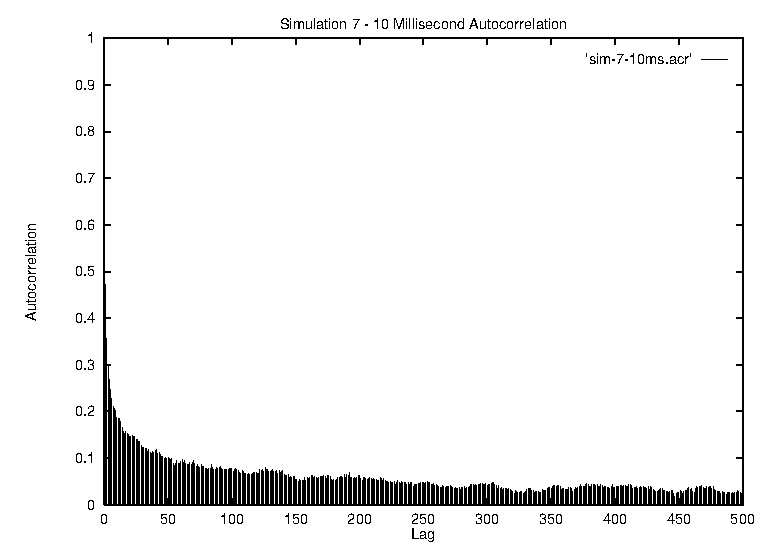
\includegraphics[height=3in]{pics/sim-7-10ms-acr.eps}
\caption{Autocorrelation of Single $t_2-distribution$ Distributed Renewal Process Simulation}
\label{simulation:sim7.10ms.acr}
\end{figure}

\begin{figure}
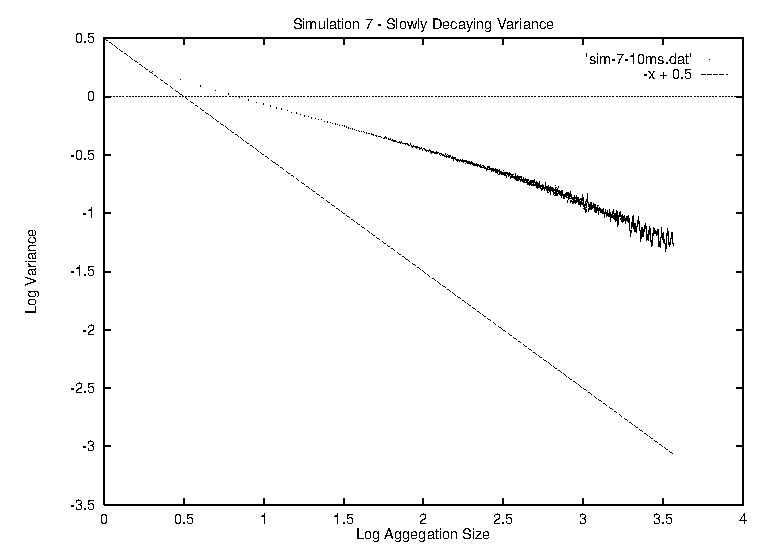
\includegraphics[height=3in]{pics/sim-7-10ms-sta.eps}
\caption{Slowly decaying variance plot of Single $t_2-distribution$ Distributed Renewal Process Simulation}
\label{simulation:sim7.10ms.sta}
\end{figure}

\begin{figure}
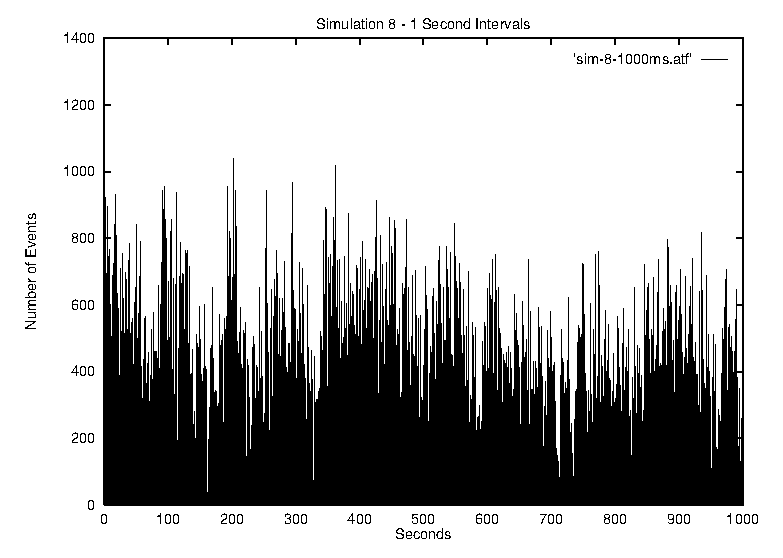
\includegraphics[height=3in]{pics/sim-8-1s-freq.eps}
\caption{10 Superimposed $t_2-distribution$ Distributed Renewal Process Simulation}
\label{simulation:sim8.1s.freq}
\end{figure}


\begin{figure}
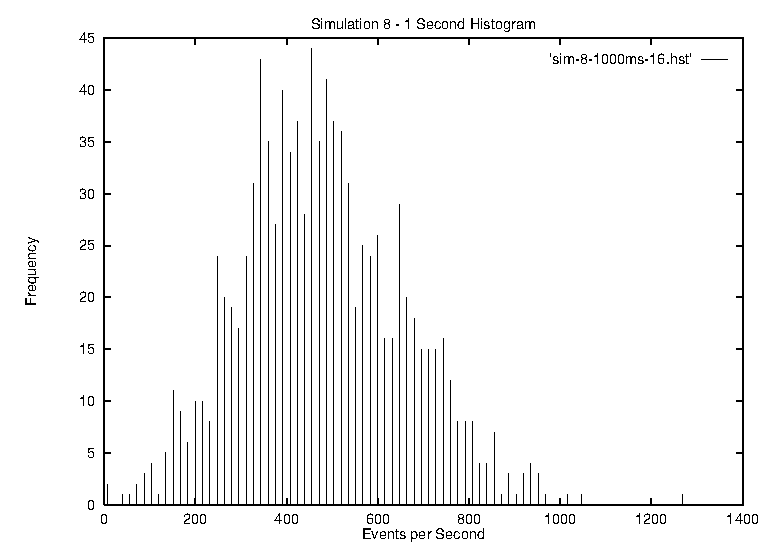
\includegraphics[height=3in]{pics/sim-8-1s-hist-16.eps}
\caption{Histogram of 10 Superimposed $t_2-distribution$ Distributed Renewal Process Simulation}
\label{simulation:sim8.1s.hist}
\end{figure}

\begin{figure}
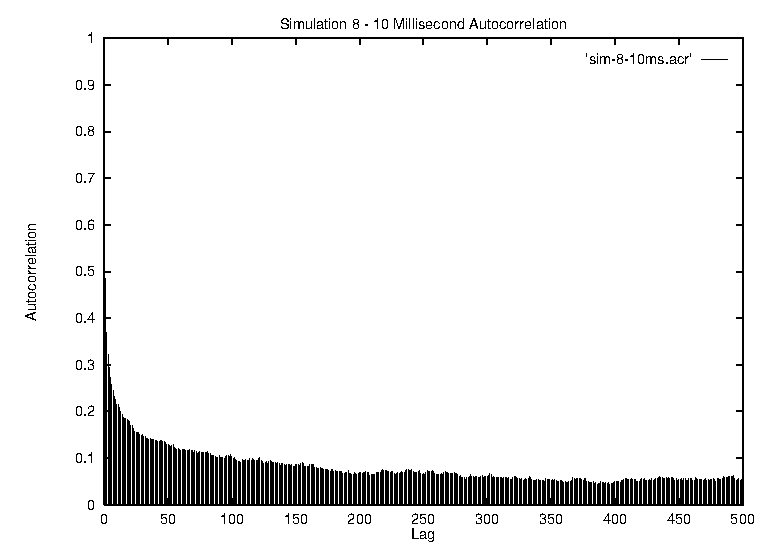
\includegraphics[height=3in]{pics/sim-8-10ms-acr.eps}
\caption{Autocorrelation of 10 Superimposed $t_2-distribution$ Distributed Renewal Process Simulation}
\label{simulation:sim8.10ms.acr}
\end{figure}

\begin{figure}
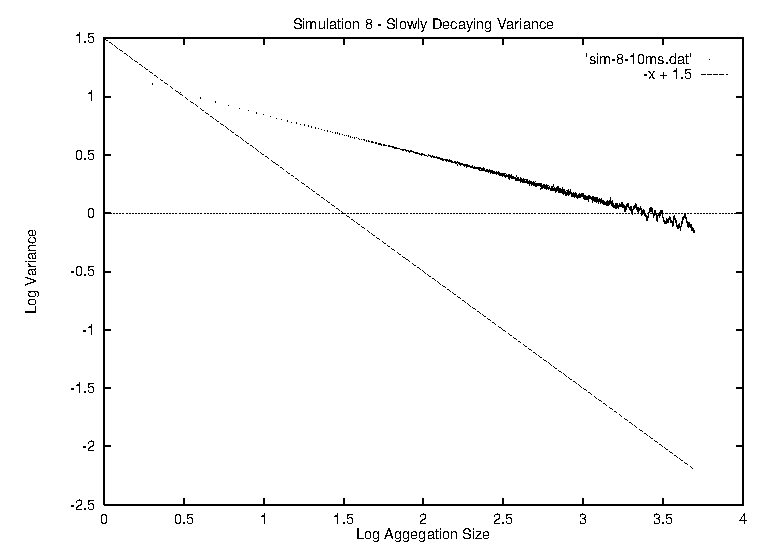
\includegraphics[height=3in]{pics/sim-8-10ms-sta.eps}
\caption{Slowly decaying variance plot of 10 Superimposed $t_2-distribution$ Distributed Renewal Process Simulation}
\label{simulation:sim8.10ms.sta}
\end{figure}

\begin{figure}[h]
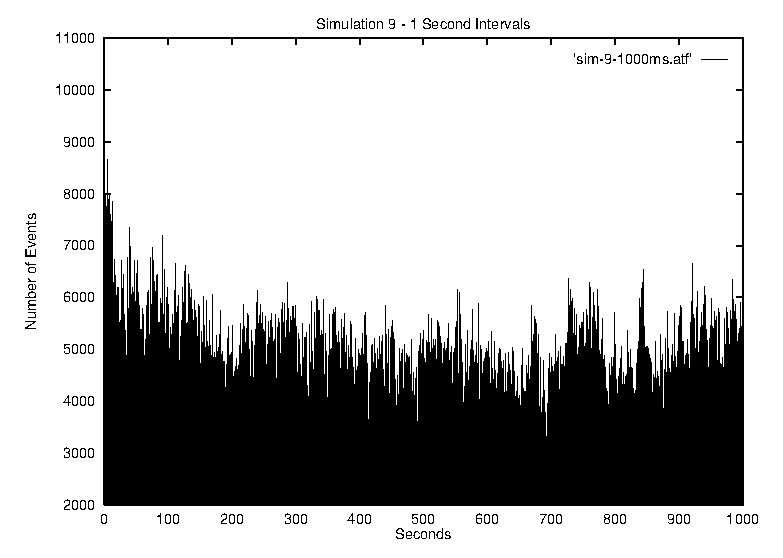
\includegraphics[height=3in]{pics/sim-9-1s-freq.eps}
\caption{100 Superimposed $t_2-distribution$ Distributed Renewal Process Simulation}
\label{simulation:sim9.1s.freq}
\end{figure}


\begin{figure}
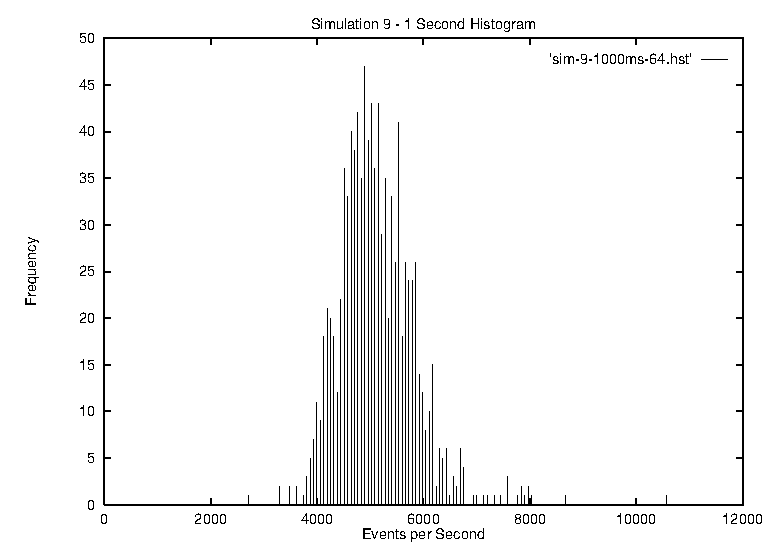
\includegraphics[height=3in]{pics/sim-9-1s-hist-64.eps}
\caption{Histogram of 100 Superimposed $t_2-distribution$ Distributed Renewal Process Simulation}
\label{simulation:sim9.1s.hist}
\end{figure}

\begin{figure}
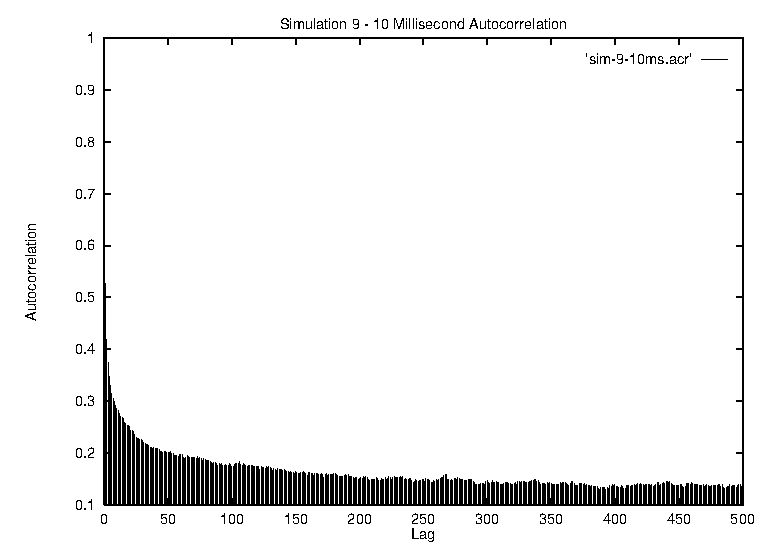
\includegraphics[height=3in]{pics/sim-9-10ms-acr.eps}
\caption{Autocorrelation of 100 Superimposed $t_2-distribution$ Distributed Renewal Process Simulation}
\label{simulation:sim9.10ms.acr}
\end{figure}

\begin{figure}
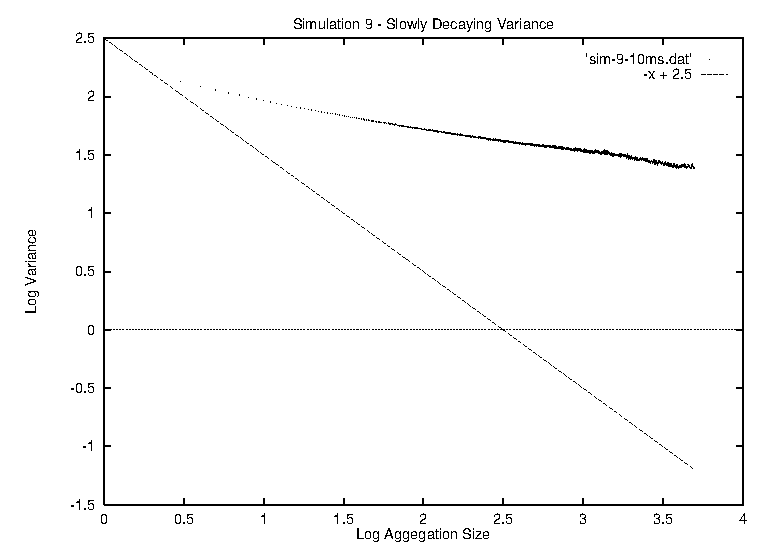
\includegraphics[height=3in]{pics/sim-9-10ms-sta.eps}
\caption{Slowly decaying variance plot of 100 Superimposed $t_2-distribution$ Distributed Renewal Process Simulation}
\label{simulation:sim9.10ms.sta}
\end{figure}

The results show that superimposing does affect slowly decaying
variance and that the number of merged processes directly influences
the rate of variance decay.

The simulations make it plain that visual inspection of the trace is
not enough.  This is clearly seen in comparing simulation 3 (general
modulated renewal process) with simulation 8 (10 merged
$t_2-distribution$ renewal processes).  While their time series
(figures
\ref{simulation:sim3.1s.freq} and \ref{simulation:sim8.1s.freq}) and
histograms (figures \ref{simulation:sim3.1s.hist} and
\ref{simulation:sim8.1s.hist}) look similar this is clearly shown to be
superficial as simulation 8 displays marked fractal properties,
whereas simulation 3 shows little beyond a Poisson process.

Although the slope of the slowly decaying plot decreases as the number
of merged processes increases, these suggest that a single process (as
for figures \ref{simulation:sim4.10ms.sta},
\ref{simulation:sim5.10ms.sta}, \ref{simulation:sim6.10ms.sta} and
\ref{simulation:sim7.10ms.sta}) is sufficient to produce time series
having self-similar behaviour.  This is a much simpler simulation than
that suggested in reference \cite{Bell:1} \cite{Bell:2} \cite{Bell:3}
\cite{Bell:4} \cite{Bell:5}.
